\documentclass[letterpaper,12pt]{article} %tipo de documento y tama~o de papel y letra
\usepackage[latin1]{inputenc} %codificacion de caracteres
\usepackage[spanish]{babel} %idioma
\usepackage{fancyhdr} %tipo de pagina, LINDA biggrin.gif
\usepackage[top=3.5cm,bottom=2.5cm,right=2cm,left=2.5cm]{geometry} %margenes
\usepackage[rflt]{floatflt} %ni puta idea
\usepackage{pdfpages} %incluir archivos pdf
\usepackage{float}
\usepackage{hyperref} %hipervinculos
\hypersetup{
  colorlinks=true,
  urlcolor=cyan
}
%\usepackage{helvet} %esto es pa escribir con Arial en vez de times new roman
%\renewcommand\familydefault{\sfdefault} %descomenta estas lineas para escribir en arial

\usepackage{multirow}

\usepackage{graphicx} %para usar imagenes
%\newcommand{\imgdir}{doc-img} % para meter las imagenes en una carpeta especial, tunz en la carpeta del documento tiene q ir otra que se llame 'doc-img'
\graphicspath{{./pic/}} %le dice que las imagenes estan en la carpeta de arriba

\usepackage{amsmath} %pa usar smbolos matematicos
\numberwithin{equation}{section} % pa usar ecuaciones de modo lindo
\numberwithin{figure}{section} %para agregar imagenes
\numberwithin{table}{section} %para agregar tablas

\usepackage{chngcntr}
\counterwithin{equation}{section}
\counterwithin{figure}{section}
\counterwithin{table}{section}

\usepackage{subfigure} % pa usar sub figuras



\pagestyle{fancy} %configuracion para la pagina linda
\renewcommand{\sectionmark}[1]{\markboth{}{\thesection\ \ #1}} %cambios de comentarios
\lhead{} %parte de arriba, izq
\chead{} %parte de arriba, centro
\rhead{\rightmark} %parte de arriba, derecha, le agrega la marca del capitulo
\lfoot{} %parte de abajo, izq
\cfoot{} %parte de abajo, centro
\rfoot{\thepage} %parte de abajo, derecha, va el numero de la pagina


%-------------portada---------------------------------%
\begin{document}
\begin{titlepage} %portada
\thispagestyle{empty} %borrar el formato de pagina linda
%\begin{flushleft} %alinear a la izq
\begin{center}

\includegraphics[scale=0.35]{logoUSM-DI.eps}
%\vfill
\end{center}
%\end{flushleft}

\vspace{3cm} %espacio vertical , en realidad es un enter de 2 cm
\begin{center} %centrar
{\Huge Requerimientos de Software \\
 \huge Proyecto ``\emph{V.I.Pe.R.}''\\
  \normalsize\today
}
\end{center}

\vspace{6cm}

\vfill
\begin{flushleft} %alinear derecha
Pre-Empresa: \emph{Phyrex}\\
Jefe de Proyecto: Rodrigo Fr\'{\i}as\\
Integrantes:
\begin{table}[hb]
  \begin{tabular}{lcc}
    Rodrigo Fr\'{\i}as & \texttt{\small <rodrigo.frias@alumnos.usm.cl>} & [+56 9 83988257] \\
    Celeste Bertin & \texttt{\small <celeste.bertin@alumnos.usm.cl>} &[+56 9 68410901]\\
    Patricio Carrasco &\texttt{\small <patricio.carrascod@alumnos.usm.cl>} &[+56 9 50626689]\\
    Rocio Fernandez &\texttt{\small <rocio.fernandezu@alumnos.usm.cl>} & [+56 9 62426549]\\
    Juan Avalo & \texttt{\small <juan.avalo@alumnos.usm.cl>} & [+56 9 78072458]\\
  \end{tabular}
\end{table}
\end{flushleft}
\end{titlepage}
%------------------fin de la portada --------------------%

%{\bf } %escribir en negrita

\setcounter{page}{1} %empezar enumerando la pagina 1

\tableofcontents
\newpage

\section{Ficha de Clasificaci\'on R\'apida}
\subsection{Objetivo del Proyecto} %140 caracteres
El objetivo principal del proyecto es el motivar a alumnos de ense\~nanza media a estudiar carreras de inform\'atica, adem\'as de generar una continuidad con los proyectos existentes en el DI, implementando una mascota virtual que mezcle las tecnolog\'ias de smartphone con OS Android y robot Lego Mindstoms, utilizando las funcionalidades del primero y los sensores del segundo, para generar experiencias que sean atractivas para el usuario.\\

\subsection{Resumen del Proyecto} %media pagina

\emph{V.I.Pe.R.}, busca mezclar distintos tipos de tecnolog\'ias para su llegada al usuario.\\

Es una mascota virtual, desarrollada en smartphone con OS Android, que busca interactuar con el usuario final, a trav\'es de las distintas funcionalidades que poseen estos dispositivos (como son la pantalla t\'actil, sensores de luminosidad, giroscopio, etc.).\\

Por otro lado, \emph{V.I.Pe.R.} tambi\'en es una mascota f\'{\i}sica, correspondiente a un robot Lego Mindstorms, el cual se comunicar\'a con el smartphone a trav\'es de una conecci\'on bluetooth y realizar\'a diferentes acciones seg\'un la interacci\'on del usuario con el equipo movil.\\

Finalmente, el robot Lego Mindstorms contar\'a con sensores con los que el usuario podr\'a relacionarse directamente, de manera tal de usar el smartphone como el ``cerebro'' del robot y poder realizar interacciones de varias maneras con el usuario.\\

Todo ello enfocado a llamar la atenci\'on del usuario por las Tecnologias de la Informaci\'on, y atraerlo a carreras de Inform\'atica.\\
\subsection{Cliente}
~\\
Nombre: Jocelyn Simmonds\\
Cargo: \\
E-mail: jsimmond@inf.utfsm.cl\\
Tel\'efono: \\
Rol o Experiencia relevante al producto:

\newpage
\section{Modelo de Dominio}

Es posible apreciar el Modelo del Dominio en la figura~\ref{fig:ModeloDominio}.

\begin{figure}[H]
   \centering
     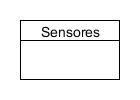
\includegraphics[scale=0.7]{ModeloDominio.jpg}
   \caption{Se puede apreciar el Modelo de Dominio relativo a \emph{V.I.Pe.R}.}
   \label{fig:ModeloDominio}
\end{figure}

Respecto a las entidades mostradas en~\ref{fig:ModeloDominio} la descripci\'on de cada una de ellas se muestra a continuaci\'on:\\

\begin{table}[H]
  \centering
  \begin{tabular}{p{5cm}p{9cm}}\hline
    Entidad & Descripci\'on \\ \hline \hline %1 linea
    Usuario & Representa a quien va a ocupar la aplicaci\'on (Un alumno, por ejemplo). \\ \hline
    Encargado & Es el que se encarga de mantener al robot y obtener los datos necesarios para difusion. \\ \hline
    Smartphone & Maneja las interacciones entre el usuario y la mascota. \\ \hline
    Mascota Virtual & Representa el ``cerebro'' de la mascota. \\ \hline
    Robot & Es el robot f\'isico, con las capacidades que tienen que estar almacenadas si o si en \'el. \\ \hline
    Motores & Representa a los motores que permiten que el robot se mueva. \\ \hline
    Brick & Representa a la unidad de control del robot. \\ \hline
    Sensores & Representan a los sensores que puede poseer el robot y que le permiten obtener informacion del ambiente. \\ \hline \hline
  \end{tabular}
\end{table}

\newpage
\section{Actores y Tareas Clave}

En la tabla siguiente, se puede apreciar la lista de los actores identificados en el proyecto.\\

\begin{table}[H]
  \centering
  \begin{tabular}{p{5cm}p{9cm}}\hline
    Actor & Descripci\'on \\ \hline \hline %1 linea
    Usuario & interactuar\'a con el animal simulado \\ \hline
    Encargado de Robot & obtendr\'a datos acerca del uso del softwware \\ \hline \hline
  \end{tabular}
\end{table}

Y a continuaci\'on, se observa la lista de tareas clave correspondientes al mismo.\\

\begin{table}[H]
  \centering
  \begin{tabular}{p{5cm}p{9cm}}\hline
    Tarea Clave & Descripci\'on \\ \hline\hline %max 3 lineas
    Crear nueva mascota & Crea una nueva mascota a gusto del usuario. \\ \hline
    Parear smartphone con robot & Conectar el dispositivo con el robot. \\ \hline
    Interactuar con smartphone & El usuario interact\'ua con la mascota que se encuentra en el tel\'efono. \\ \hline
    Interactuar con robot & El usuario activa sensores en el animal f\'isico, generando una interacci\'on entre ellos. \\ \hline
    Recolectar informaci\'on del robot & El encargado del robot obtiene datos estad\'asticos sobre el uso de la aplicaci\'on por los usuarios. \\ \hline\hline
  \end{tabular}
\end{table}

\newpage
\section{Requerimientos Extra-funcionales}

No se aprecian requerimientos extra-funcionales que sean importantes para el proyecto.\\

%\begin{table}[H]
%  \centering
%  \begin{tabular}{lp{9cm}}\hline 
%    Req. Extra-funcional & Descripci\'on y medici\'on \\ \hline\hline %max 2 lineas
%    & \\ \hline
%  \end{tabular}
%\end{table}

\newpage
\section{Restricciones de Software y Hardware}

A continuaci\'on se detallan las restricciones propias del Software y del Hardware, tanto en las limitantes de comunicaci\'on entre ellos, como en lo solicitado por el cliente.\\

\begin{table}[H]
  \centering
  \begin{tabular}{p{5cm}p{9cm}}\hline
    Restricci\'on & Raz\'on \\ \hline\hline %max 2 lineas
    Sistema rob\'otico debe ser LEGO Mindstorm NXT & Herramienta para principiantes, permite mayor manipulaci\'on y dinamicidad a la construcci\'on, adem\'as de ser atractivo para el usuario.\\ \hline
    Aplicaci\'on m\'ovil debe programarse para smartphones con OS Android & Facilidad en la disponibilidad del recurso de trabajo. \\ \hline
    Conectividad entre mascota f\'isica y aplicaci\'on debe ser por bluetooth & Resulta de las restricciones anteriores. Es la tecnolog\'{\i}a que tienen en com\'un para comunicarse entre ellos.\\ \hline \hline
  \end{tabular}
\end{table}

\newpage
\section{Casos de Uso} %al menos 3 casos de uso no-triviales

En la figura~\ref{fig:CasoUso}, se puede apreciar los casos de uso del proyecto, englobando algunos en un nivel de abstracci\'on alto como son los casos de interacci\'on, ya sea con el smartphone o con el robot.\\

\begin{figure}[H]
   \centering
     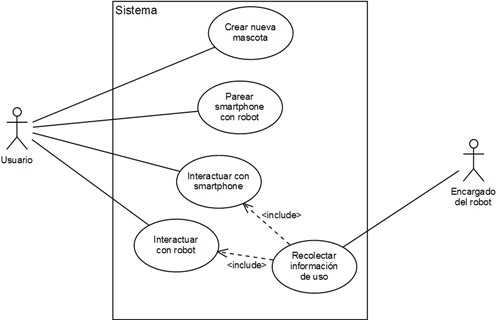
\includegraphics[scale=1]{CasoUso.jpg}
   \caption{Es posible apreciar algunos Casos de Uso relativos al proyecto \emph{V.I.Pe.R.}.}
   \label{fig:CasoUso}
\end{figure}

Respecto a los casos de uso no-triviales, cabe destacar tres que son necesarios para la aplicaci\'on, en distintos niveles de aplicaci\'on. Por un lado, est\'a el caso de uso ``Crear Mascota'' que hace referencia a la interacci\'on entre usuario y el smartphone con Android, y es el que se detalla a continuaci\'on.\\

\begin{table}[H]
  \centering
  \begin{tabular}{p{5cm}p{9cm}}\hline\hline
    Nombre: & Crear Mascota. \\ \hline
    Descripci\'on: & El usuario al utilizar la aplicaci\'on Android por primera vez, debe crear una mascota virtual, que va a ser el medio de interacci\'on entre dicho dispositivo y el robot Lego Mindstorms\\ \hline %max 5 lineas
    Pre-condiciones: & No debe existir una mascota anteriormente.\\ \hline
    Post-condiciones: & Mascota Virtual creada y esperando para interactuar con el usuario\\ \hline
    Requerimientos no Funcionales: & ---\\ \hline\hline %min 0 ; max 3
  \end{tabular}
  \label{tab:Crear}
\end{table}

Luego, el segundo caso de uso se denomina ``Parear y Calibrar'', el que es posible observar m\'as en detalle en la tabla siguiente, y abarca el nivel de interacci\'on entre el equipo smarthphone y el robot Lego Mindstorms.\\

\begin{table}[H]
  \centering
  \begin{tabular}{p{5cm}p{9cm}}\hline\hline
    Nombre: & Parear y Calibrar. \\ \hline
    Descripci\'on: & Es necesario poder transmitir datos desde la aplicaci\'on Android hacia el robot y viceversa, para ello es necesario poder comunicar los equipos. Adem\'as, estos deben poder funcionar correctamente en el medio en el que se encuentran.\\ \hline %max 5 lineas
    Pre-condiciones: & Smartphone Android y Robot Lego Mindstorms no pareados (sin comunicaci\'on entre ellos).\\ \hline
    Post-condiciones: & Smartphone Android y Robot Lego Mindstorms pareados (con comunicaci\'on entre uno y otro) y con la funcionalidad correspondiente al medio en que se encuentre el robot (fuerza de los motores seg\'un terreno, sensibilidad de sensores, etc.)\\ \hline
    Requerimientos no Funcionales: &
    \begin{itemize}
    \item Disponer de al menos 3 niveles de fuerza en motores encargados de movimiento.
    \end{itemize}\\ \hline\hline %min 0 ; max 3
  \end{tabular}
  \label{tab:Parear}
\end{table}

Finalmente tenemos el caso de uso ``Recolectar informaci\'on de uso'', que hace referencia al \'ambito de interacci\'on del caso anterior, pero para un posterior uso del ``Encargado del Robot''.\\

\begin{table}[H]
  \centering
  \begin{tabular}{p{5cm}p{9cm}}\hline\hline
    Nombre: & Recolectar informaci\'on de uso.\\ \hline
    Descripci\'on: & Debido al objetivo en cuanto a difusi\'on, se hace necesario saber que tipo de futuros alumnos est\'an utilizando el sistema, y que tipo de uso se le da al mismo.\\ \hline %max 5 lineas
    Pre-condiciones: & ``Parear y Calibrar'', Usuario interactuando con el sistema.\\ \hline
    Post-condiciones: & Datos de uso de las funcionalidades de la aplicaci\'on.\\ \hline
    Requerimientos no Funcionales: & ---\\ \hline\hline %min 0 ; max 3
  \end{tabular}
  \label{tab:Recolectar}
\end{table}


\end{document}
